%% =====================================================================
%% Final Report -- AI in Cellular Communication (Fall 2026)
%% AI-Driven Beam Management for 6G: A Survey with a Digital Twin Case Study
%% Template: IEEEtran (journal). Limit: 5 pages. Due: 15-Dec-2026, 18:00.
%% Author: Maria Munoz, University of Seoul.
%% Compile: pdflatex main && bibtex main && pdflatex main && pdflatex main
%% =====================================================================
\documentclass[journal]{IEEEtran}
\usepackage{cite}
\usepackage{amsmath,amssymb}
\usepackage{graphicx}
\usepackage{booktabs}
\usepackage{multirow}
\usepackage{url}
\usepackage[hidelinks]{hyperref}
\graphicspath{{../figures/paper/}}

\begin{document}
\bstctlcite{IEEEexample:BSTcontrol}

\title{AI-Driven Beam Management for 6G:\\ A Survey with a Digital Twin Case Study}

\author{Mar\'ia~Mu\~noz
\thanks{M.~Mu\~noz is with the University of Seoul, Seoul, Korea (e-mail: mariamunors@gmail.com). Report for the course \emph{AI in Cellular Communication}, Fall 2026.}}

\markboth{AI in Cellular Communication -- Final Report}{}
\maketitle


% ---------------------------------------------------------------------
\begin{abstract}
Large antenna arrays in 5G-Advanced and 6G form narrow beams, and finding the best one by exhaustive sweeping costs time, energy and reference signals. This paper surveys AI-driven beam management: position-aided, measurement-aided (3GPP BM-Case~1), sensing-aided and temporal (BM-Case~2) prediction, and its standardization in 3GPP Releases~18 and~19. We also build a ray-tracing digital twin of the University of Seoul campus with Sionna~RT and OpenStreetMap and evaluate the main families at 3.5 and 4.7~GHz. Pointing the beam at the user's position loses 6~dB on average; a neural network using the position stays below 1~dB while testing 4 of 32 beams, and position plus four measured beams reaches 77\,\% top-1 accuracy and a 0.12~dB loss with 8 beams. For a walking user, AI prediction with 7 beams per step loses less than half as much as a delayed full sweep. We close with open challenges in generalization, data and life-cycle management.
\end{abstract}

\begin{IEEEkeywords}
Beam management, deep learning, digital twin, ray tracing, 3GPP, 5G-Advanced, 6G.
\end{IEEEkeywords}

% =====================================================================
\section{Introduction}
\IEEEPARstart{M}{assive} antenna arrays are central to 5G and 6G: at millimeter-wave frequencies they compensate for the high path loss, and in the mid-band they increase capacity. The price is that the energy is concentrated in narrow beams that must be pointed at each user. In 5G New Radio this is done by \emph{beam management}: the base station (gNB) sweeps a codebook of beams, the user equipment (UE) measures them and reports the best one~\cite{giordani2019tutorial}. The overhead of this sweep grows with the size of the codebook, and the procedure must be repeated whenever the user moves, turns or is blocked, which makes beam management one of the key challenges for 5.5G and 6G systems~\cite{heng2021six}.

Artificial intelligence (AI) offers a different approach. The best beam at a given location is largely determined by the surrounding buildings and reflectors, so a model trained on past data can predict it from cheap side information (position, a few measurements, camera images or the history of the user) and the network only needs to verify a small set of candidates~\cite{ma2023dlbm,xue2024survey}. The idea has moved quickly from research to standardization: 3GPP studied AI/ML for the NR air interface in Release~18, with beam management as one of three use cases~\cite{3gpp38843}, and Release~19 turns it into normative work~\cite{3gppRel19}.

Existing surveys on beam management are broad and long~\cite{xue2024survey}. This report gives a compact overview, complemented by a case study in a real environment built with open tools, in the spirit of the digital twins proposed for 6G~\cite{alkhateeb2023twins}. Its contributions are: (i) a taxonomy and comparison of AI-based beam management works (Table~\ref{tab:works}); (ii) a summary of the 3GPP framework; and (iii) a digital-twin case study of the University of Seoul (UOS) campus at 3.5 and 4.7~GHz that evaluates position-aided, measurement-aided and temporal prediction under the same conditions. Sections~\ref{sec:fund}--\ref{sec:std} cover fundamentals, AI techniques and standardization, Section~\ref{sec:case} the case study, and Section~\ref{sec:open} open challenges.

% =====================================================================
\section{Beam Management Fundamentals}
\label{sec:fund}
\subsection{The NR Procedure}
NR beam management is organized in three phases~\cite{giordani2019tutorial}. In P1 the gNB sweeps wide beams carried by synchronization signal blocks (SSBs) and the UE reports the strongest ones; in P2 the gNB refines the selection with narrower beams using channel state information reference signals (CSI-RS); in P3 the UE adjusts its own receive beam. Each step relies on layer-1 reference signal received power (L1-RSRP) measurements, and each measured beam consumes time-frequency resources, latency and UE power.

\subsection{Problem Formulation}
Let $\mathbf{h}\in\mathbb{C}^{M}$ be the channel between an $M$-antenna gNB and a single-antenna UE, and let $\mathcal{A}=\{\mathbf{w}_1,\dots,\mathbf{w}_N\}$ be the beam codebook (Set~A in 3GPP terminology). The best beam is
\begin{equation}
k^\star=\arg\max_{k\in\{1,\dots,N\}} \left|\mathbf{h}^{\mathsf H}\mathbf{w}_k\right|^2 .
\end{equation}
An exhaustive sweep measures all $N$ beams. AI-based beam management instead measures a small Set~B ($|\mathcal{B}|\ll N$), possibly complemented with side information, and predicts $k^\star$ or a short list of candidates that are then measured.

\subsection{Performance Metrics}
The literature and 3GPP evaluations use three main metrics~\cite{3gpp38843,xue2023standard}: the top-$K$ accuracy (probability that $k^\star$ is among the $K$ predicted beams), the RSRP or power loss in dB of the selected beam with respect to $k^\star$, and the measurement overhead reduction, $1-|\mathcal{B}|/N$. The power loss is often more informative than accuracy, because choosing a neighbouring beam may cost only a fraction of a decibel.

\subsection{Why Beam Management Is Hard}
The best beam changes abruptly when the line of sight is blocked and a reflection becomes dominant, when the user moves or rotates, and, in wideband systems, when the beam direction varies across the band (beam squint)~\cite{heng2021six}. Geometry alone, i.e., pointing the beam towards the user, therefore fails in non-line-of-sight areas, as our case study confirms in Section~\ref{sec:case}.

% =====================================================================
\section{AI Techniques for Beam Management}
\label{sec:ai}
Table~\ref{tab:works} summarizes representative works. We group them by the information they use as input.

\subsection{Position-Aided Prediction}
Since the propagation environment is mostly static, the UE position is a strong predictor of the best beam. Va~\emph{et al.}~\cite{va2018inverse} proposed \emph{inverse multipath fingerprinting}: a database indexed by position stores the beams that worked in the past, and only those candidates are trained, which outperforms standard beam training when the arrays grow. Morais~\emph{et al.}~\cite{morais2023position} evaluated position-aided prediction on real measurements from nine DeepSense~6G scenarios and compared neural networks, $k$-nearest neighbours (kNN) and lookup tables. They found that simple methods perform similarly to neural networks and that the accuracy is limited by the noise of the GPS positions.

\subsection{Prediction from Partial Beam Measurements}
In the spatial-domain case (3GPP BM-Case~1) the UE measures a Set~B and a model infers the quality of all beams in Set~A. Echigo~\emph{et al.}~\cite{echigo2021low} treated this as a ``super-resolution'' problem and used convolutional networks to estimate all beam qualities from a few measurements taken with codebooks of different widths. A related idea uses out-of-band information: Alrabeiah and Alkhateeb~\cite{alrabeiah2020sub6} showed that sub-6~GHz channels can predict the best mmWave beam and detect blockage with more than 90\,\% accuracy. 3GPP-style evaluations confirm the gains: in~\cite{xue2023standard}, AI raises the top-1 accuracy from 10.7\,\% to 63.5\,\% and reduces the RSRP difference from 4.22 to 0.36~dB with respect to selecting the best measured beam, and in~\cite{jayaweera2024bm} BM-Case~1 reaches 75--95\,\% top-1 accuracy depending on the size of Set~B, with 50--87.5\,\% fewer measurements.

\subsection{Sensing-Aided and Multi-Modal Prediction}
Cameras, LiDAR and radar provide information about the user and the blockers that radio measurements alone cannot. Charan~\emph{et al.}~\cite{charan2022vision} fused camera images and position on real data and obtained more than 75\,\% top-1 and almost 100\,\% top-3 accuracy. These works are enabled by large real-world datasets such as DeepSense~6G, which combines camera, LiDAR, radar, GPS and per-beam power measurements~\cite{alkhateeb2023deepsense}. The drawback is the extra hardware and the privacy concerns of cameras.

\subsection{Temporal Prediction and Beam Tracking}
For moving users, the temporal-domain case (BM-Case~2) uses the history of measurements to predict the future best beam, so that the beam can be switched before the link degrades. Jiang and Alkhateeb~\cite{jiang2022tracking} used sequences of images to predict future beams in a real deployment, reaching 64.5\,\% top-1 accuracy and 97.7\,\% of the optimal power with less than 1\,\% of the beam training overhead. In the 3GPP-style evaluation of~\cite{jayaweera2024bm}, BM-Case~2 obtains 59--91.5\,\% top-1 accuracy within a 1~dB margin, but the performance depends on the user speed. Recurrent networks (LSTM, GRU) are the most common models for this task.

\subsection{Data: Ray Tracing, Datasets and Digital Twins}
All these models need large amounts of labelled data, which are expensive to measure. Ray tracing was used early on to generate datasets for beam selection, e.g., Raymobtime~\cite{klautau2018data}. Alkhateeb~\emph{et al.}~\cite{alkhateeb2023twins} go further and propose real-time digital twins that combine 3D maps, sensing and ray tracing to train and test models before and during deployment. Differentiable ray tracers such as Sionna~RT~\cite{hoydis2023sionnart} make it possible to calibrate the twin with measurements, and tools such as SceneBaker~\cite{lyu2026scenebaker} build radio-ready scenes directly from OpenStreetMap.

\subsection{Comparison}
Position-aided methods need the least signalling but depend on accurate positioning; measurement-based methods reuse existing reference signals and fit the 3GPP framework; sensing-aided methods excel in dynamic scenes but need extra hardware; temporal models are essential for mobility but sensitive to speed. In all cases, generalization to new sites is the main weakness.

\begin{table*}[!t]
\caption{Representative AI-Based Beam Management Works}
\label{tab:works}
\centering
\footnotesize
\renewcommand{\arraystretch}{1.12}
\begin{tabular}{@{}l l l l p{6.4cm}@{}}
\toprule
Ref. & Family (3GPP case) & Input & Data & Key idea / reported result \\
\midrule
\cite{va2018inverse} & Position-aided & UE position & Ray tracing (V2I) & Position-indexed multipath fingerprint database selects candidate beams; outperforms IEEE 802.11ad training as arrays grow. \\
\cite{morais2023position} & Position-aided & GPS position & Real (DeepSense 6G) & Compares NN, kNN and lookup tables on 9 real scenarios; position noise limits accuracy. \\
\cite{echigo2021low} & Partial meas. (BM-1) & Subset of beams & Simulation & CNN/ConvLSTM ``super-resolution'' of beam qualities from few measurements with multi-width codebooks. \\
\cite{alrabeiah2020sub6} & Out-of-band & Sub-6 GHz channel & Ray tracing & Maps sub-6 GHz CSI to the best mmWave beam and to blockage ($>$90\,\% blockage prediction). \\
\cite{charan2022vision} & Sensing-aided & Camera + position & Real (DeepSense 6G) & Multi-modal fusion: $>$75\,\% top-1 and $\approx$100\,\% top-3 accuracy. \\
\cite{jiang2022tracking} & Temporal (BM-2) & Camera sequence & Real (DeepSense 6G) & Future-beam prediction: 64.5\,\% top-1, 97.7\,\% normalized power, $<$1\,\% of training overhead. \\
\cite{jayaweera2024bm} & BM-1 and BM-2 & Set B RSRP & 3GPP system-level & Rel-18 evaluation: 75--95\,\% top-1 (BM-1); 59--91.5\,\% top-1 within 1 dB (BM-2). \\
This work & Position, BM-1, BM-2 & Position, Set B & Ray-traced campus twin & UOS digital twin at 3.5/4.7 GHz: 77\,\% top-1 and 0.12 dB loss with 8 of 32 beams. \\
\bottomrule
\end{tabular}
\end{table*}

% =====================================================================
\section{Standardization in 3GPP}
\label{sec:std}
The Release~18 study item on AI/ML for the NR air interface, documented in TR~38.843~\cite{3gpp38843}, selected three pilot use cases: CSI feedback, beam management and positioning. For beam management it defined two sub-use cases~\cite{xue2023standard}. In BM-Case~1 (spatial prediction), the best beams of Set~A are predicted from measurements of Set~B at the same time instant; Set~B can be a subset of Set~A or a different set of wider beams. In BM-Case~2 (temporal prediction), the best beams at future instants are predicted from the history of Set~B measurements.

The study also considered where the model runs (UE or network side) and introduced \emph{life-cycle management} (LCM): data collection, training, inference, performance monitoring, and model switching or fallback~\cite{xue2023standard,gao2026rel19}. LCM is needed because a model trained in one scenario can silently degrade in another: the top-1 accuracy can drop by 25\,\% or more when the antenna configuration changes, and performance also degrades when the UE speed differs from the training data~\cite{jayaweera2024bm}.

Release~19 started normative work on AI/ML for beam management, together with positioning and CSI prediction~\cite{3gppRel19,gao2026rel19}. Release~20 hosts the 6G studies and Release~21 is expected to contain the first 6G specifications~\cite{3gppRel19}. Since the standard leaves model design to vendors, cheap and realistic training data become essential, which motivates the digital-twin case study below.

% =====================================================================
\section{Case Study: A Digital Twin of the University of Seoul}
\label{sec:case}

\subsection{Digital Twin and Dataset}
We built a ray-tracing digital twin of the University of Seoul (UOS) campus and its surroundings ($1.2\times1.1$~km). Buildings, roads and vegetation were taken from OpenStreetMap together with SRTM terrain, and converted into a Sionna~RT scene with SceneBaker~\cite{lyu2026scenebaker,hoydis2023sionnart}; buildings without height information were assigned 15~m. A gNB was placed 3~m above the highest rooftop on campus, at the foot of Mt.~Baebong, with a $1\times16$ uniform linear array ($\lambda/2$ spacing, 3GPP TR~38.901 element pattern) oriented towards the campus centroid. Beamforming uses a DFT codebook of $N=32$ beams steered from $-60^\circ$ to $+60^\circ$ (Set~A). For every beam, the received power was ray-traced (up to five interactions, including diffraction) on a $4\times4$~m grid that follows the terrain at a handset height of 1.5~m. Cells with path gain above $-130$~dB inside the $\pm60^\circ$ sector form the dataset (about 29\,000 locations). The experiment was repeated at 3.5~GHz (public 5G, band n78) and at 4.7~GHz, the band used by Korean private 5G (e-Um 5G) networks.

To evaluate generalization to unseen areas, the campus was divided into $40\times40$~m blocks, and 70\,/\,15\,/\,15\,\% of the blocks were used for training, validation and testing. A random split would leak information between neighbouring cells and overestimate accuracy.

\subsection{Why Geometry Is Not Enough}
Fig.~\ref{fig:maps}(a) shows the best beam at every location. Close to the gNB the beams form clean angular sectors, but behind buildings the best beam often points towards a reflecting facade instead of the user. Pointing the beam straight at the user's position (the \emph{geometric beam}) selects a different beam in 31\,\% of the locations and loses 6.1~dB on average with respect to an exhaustive sweep, with a 90th percentile of 20.4~dB (Fig.~\ref{fig:maps}(b)). Site-specific learning is therefore needed.

\begin{figure*}[!t]
\centering
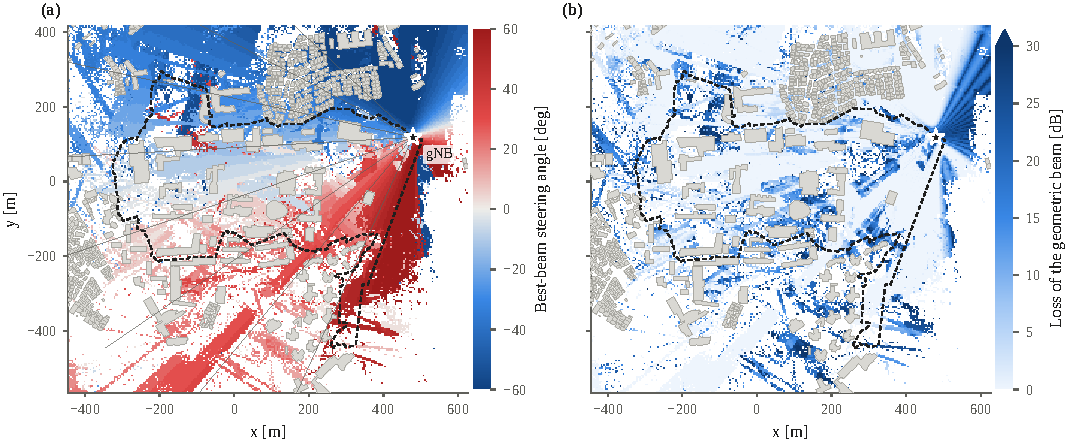
\includegraphics[width=\textwidth]{fig1_beam_maps}
\caption{UOS digital twin at 3.5~GHz. (a) Steering angle of the best of 32 beams at each location; thin lines show every fourth beam direction. (b) Power loss of the geometric beam (pointing straight at the user) with respect to the exhaustive sweep. Dashed line: campus boundary; star: gNB.}
\label{fig:maps}
\end{figure*}

\subsection{Predictors}
\emph{Position only.} A multilayer perceptron (three hidden layers of 256 units) maps the user position to a score per beam. The input is expanded with Fourier features $[\sin(2^k\pi\mathbf{p}),\cos(2^k\pi\mathbf{p})]_{k=0}^{2}$, which let a small network represent the sharp beam boundaries created by buildings~\cite{tancik2020fourier}. It is trained with soft labels (softmax of the per-beam gains with a 2~dB temperature) and compared with the geometric beam and a $k$-nearest-neighbour lookup ($k=5$), the baselines used in~\cite{morais2023position}. The UE then measures the top-$k$ predicted beams and keeps the strongest.

\emph{Position + Set~B (BM-Case~1).} The UE first measures a Set~B of 4 (or 8) uniformly spaced beams of Set~A with 1~dB measurement error; the network receives these measurements, optionally with the position.

\emph{Walking user (BM-Case~2).} A two-layer GRU observes the last four steps (4~m each, about 3~s at walking speed) of position and Set~B measurements and predicts the best beam at the next step. It is compared with a full 32-beam sweep whose result is applied one step later.

\subsection{Results}
Fig.~\ref{fig:pred}(a) shows the mean loss on unseen blocks versus the number of beams tested. With position only, the neural network and kNN reach a similar top-1 accuracy (55\,\% and 57\,\%), both clearly above the geometric beam (48\,\%), in line with the real-world observations of~\cite{morais2023position}. When a few candidates are tested, the network ranks them better: it stays below 1~dB with 4 of 32 beams (an 88\,\% reduction of the sweep) and reaches 0.22~dB with 8 beams, versus 0.49~dB for kNN and 1.41~dB for the geometric beam.

Measuring a small Set~B without AI is ineffective with narrow beams: keeping the strongest of 4 measured beams loses 10.6~dB. Feeding the same measurements to a network raises the top-1 accuracy to 72\,\%, and adding the position raises it to 77\,\%; with 8 beams measured in total the loss is only 0.12~dB, almost the performance of the exhaustive 32-beam sweep (Fig.~\ref{fig:pred}(b)). With 8 measured beams the top-1 accuracy reaches 88\,\% and the position no longer adds information. At very low overhead (5 beams) position alone performs as well as position plus four measurements, i.e., the digital-twin position is worth roughly four beam measurements.

\begin{figure*}[!t]
\centering
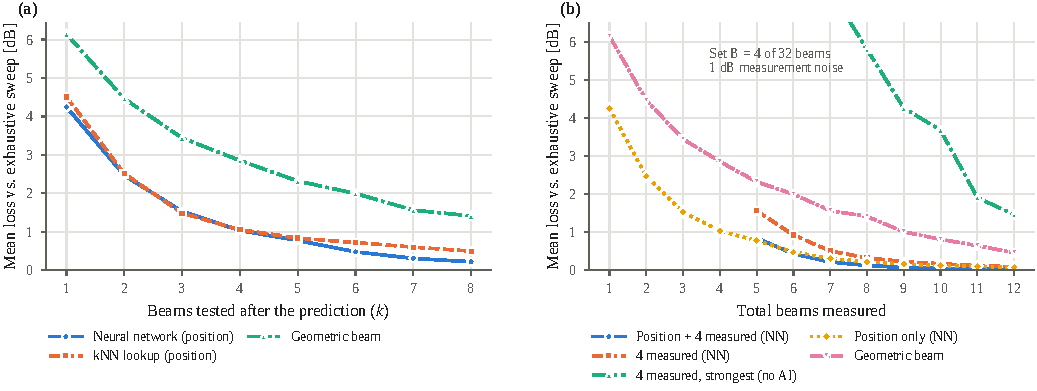
\includegraphics[width=\textwidth]{fig2_beam_prediction}
\caption{Mean power loss with respect to the exhaustive sweep on unseen campus areas (3.5~GHz). (a) Position-only prediction versus the number of predicted beams tested. (b) 3GPP BM-Case~1: Set~B of 4 beams (1~dB measurement error) plus the predicted beams, versus the total number of beams measured.}
\label{fig:pred}
\end{figure*}

For the walking user (Fig.~\ref{fig:walk}), the full sweep applied one step late loses 3.2~dB because the best beam changes while the user moves. The AI schemes measure only 7 beams per step (Set~B plus the top-3 predicted beams) and lose 1.3~dB; the GRU memory brings a small additional gain over a predictor that sees only the current step.

Finally, Fig.~\ref{fig:freq} compares both bands. At 4.7~GHz the mean best-beam path gain is 2.5~dB lower, which matches the expected free-space difference $20\log_{10}(4.7/3.5)=2.56$~dB, but the beam structure is set by the campus geometry and the array, so all predictors keep the same accuracy (Table~\ref{tab:results}). Only temporal prediction degrades slightly (1.55 vs.\ 1.25~dB).

\begin{figure}[!t]
\centering
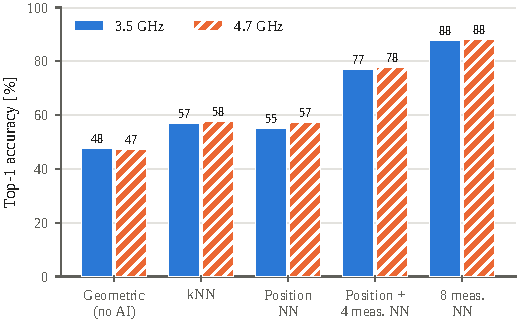
\includegraphics[width=0.88\columnwidth]{fig3_frequency}
\caption{Top-1 accuracy on unseen areas at 3.5~GHz (public 5G) and 4.7~GHz (Korean private 5G).}
\label{fig:freq}
\end{figure}

\begin{figure}[!t]
\centering
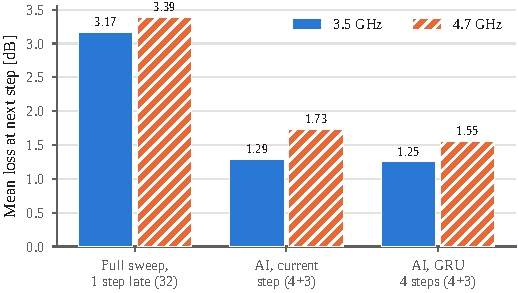
\includegraphics[width=0.88\columnwidth]{fig4_walking_user}
\caption{Walking user: mean loss of the beam used at the next step. Numbers in brackets: beams measured per step.}
\label{fig:walk}
\end{figure}

\begin{table}[!t]
\caption{Case-Study Summary on Unseen Areas}
\label{tab:results}
\centering
\footnotesize
\begin{tabular}{@{}lcc@{}}
\toprule
Metric & 3.5 GHz & 4.7 GHz \\
\midrule
Best beam $\neq$ geometric beam & 31.2\,\% & 31.9\,\% \\
Loss of geometric beam & 6.05 dB & 6.25 dB \\
Position NN, top-1 & 54.9\,\% & 57.4\,\% \\
Position NN, loss with 4 beams & 1.03 dB & 1.14 dB \\
Position + 4 meas., top-1 & 77.0\,\% & 77.7\,\% \\
Position + 4 meas., loss with 8 beams & 0.12 dB & 0.12 dB \\
Walking user, GRU (7 beams/step) & 1.25 dB & 1.55 dB \\
Full sweep one step late (32/step) & 3.17 dB & 3.39 dB \\
\bottomrule
\end{tabular}
\end{table}

\subsection{Limitations}
The twin uses default building heights and generic materials, and its results have not been validated with measurements; the dataset is single-site and static (no vehicles or people), so the reported accuracy is an upper bound for a real deployment. A 3D video of the walking-user scenario, an interactive map of the predictions and the code are available from the author on request.

% =====================================================================
\section{Open Challenges and Future Directions}
\label{sec:open}
\emph{Generalization.} Models trained in one site, with one array or at one speed lose accuracy elsewhere~\cite{jayaweera2024bm}. Training on mixed datasets, fine-tuning with a few local samples and online learning are promising, but how to do this within the signalling constraints of the standard is still open~\cite{xue2023standard}.

\emph{Data and sim-to-real gap.} Real measurements are expensive, and synthetic data are only as good as the twin. Our case study uses default building heights and generic materials; calibrating such twins with a few drive tests, for instance through differentiable ray tracing, is a natural next step~\cite{alkhateeb2023twins,hoydis2023sionnart}.

\emph{Monitoring and life-cycle management.} The network must detect when a model fails and fall back to conventional sweeping. Defining reliable monitoring metrics and model identification across vendors is a key topic of the current 3GPP work~\cite{xue2023standard,gao2026rel19}.

\emph{Foundation models.} Instead of one small model per task and site, large wireless models pre-trained on many channels could be adapted to beam prediction and other tasks with little data~\cite{alikhani2024lwm}.

\emph{Sensing and private networks.} Integrated sensing and communication may provide side information without extra cameras, and campus private networks (e.g., Korean e-Um~5G at 4.7~GHz) are natural testbeds to combine a twin, measurements and AI.

% =====================================================================
\section{Conclusion}
\label{sec:concl}
This report reviewed AI-driven beam management and its standardization in 3GPP. A digital twin of the UOS campus showed that geometry alone loses 6~dB, while AI stays below 1~dB testing 4 of 32 beams, reaches 0.12~dB with position plus 8 measured beams, and halves the loss of a delayed sweep for a walking user, at both 3.5 and 4.7~GHz. AI can remove most of the sweeping overhead, and digital twins offer a cheap way to evaluate it before deployment; generalization and validation with real measurements remain the main open problems.

\bibliographystyle{IEEEtran}
\bibliography{references}

\end{document}
